
\subsection{Elastic Exposure, Rigid Assumptions}

The pitch was simple:
Tighter latency on European venues.
Flexible regulatory treatment of synthetic instruments.
Speed, at scale.

The risk?
\textit{Contained.} At least, according to the memo he just signed.

He didn’t love the language.

\begin{itemize}
    \item ``Elastic notional synthesis.'' 
    \item ``Latency-sliced positioning.'' 
    \item ``Behavior-aware hedging.''
\end{itemize}

It read like a PowerPoint built for people who liked the sound of algorithms more than the 
feel of them.

But it wasn’t his call anymore.

David had scoped the model with his team, built it to breathe in narrow bands, and calibrated it for edge 
cases and gentle undulations.
It wasn’t built for speed.
It was built for resilience.

He’d insisted on constraints early — not because they looked good in a compliance deck, but because 
he knew what happened to models that grew too fast without discipline. They didn’t crash noisily. 
They drifted. They wandered from their training boundaries, mistaking correlation for cause, 
extrapolating patterns from noise.

So he made the team do it the hard way.
Stress it. Squeeze it. Make it learn how to be wrong — gently.

The model wasn’t optimized to chase alpha in every tick.
It was built to survive the whiplash.
To know when to hold, when to hedge, and when to stop trusting its own instincts.

He’d run simulations that didn’t reward success — they penalized overconfidence.
He made sure the confidence intervals were wide where they needed to be, and shallow where assumptions 
got thin.

It didn’t always win fast.
But it didn’t overfit. It didn’t hallucinate. It didn’t panic.

He hadn’t built a sniper.
He’d built a climber. One that knew the terrain would shift beneath it — and that staying upright mattered 
more than moving first.

\medskip

\begin{TechnicalSidebar}{Why Machine Learning Models Must Be Continuously Trained}

  Machine learning models are not static assets.  
  They are probabilistic approximators—trained not to be \textit{correct}, but to be 
  \textit{informationally relevant} to the distribution they’ve seen.
  
  \medskip
  
  \textbf{But that distribution moves.}

  \medskip
  
  In trading systems, this is called \textit{non-stationarity}. In ML theory, it's 
  \textit{distributional drift}. In practical terms:  
  what worked yesterday might fail quietly tomorrow.
  
  \medskip
  
  A model trained on old market conditions may:

  \medskip
  
  \begin{itemize}
    \item Suppress signals it now considers noise
    \item Misclassify valid anomalies as benign
    \item Overfit to structural patterns that no longer exist
  \end{itemize}

  \medskip
  
  Worse: without retraining, the confidence scores remain high—even as accuracy degrades.  
  This is the most dangerous form of model failure: \textbf{not silent, but self-assured.}
  
  \medskip
  
  \textbf{Continuous retraining} isn’t a nice-to-have. It’s survival.  

  \medskip

  It requires:

  \medskip
  
  \begin{itemize}
    \item Streaming pipelines for ingesting new data
    \item Validation infrastructure that can reweight on the fly
    \item Human oversight for flagging edge-case drift before it calcifies into error
  \end{itemize}

  \medskip
  
  In theory, all models degrade.  
  In practice, only the ones that get updated stay useful.
  
\end{TechnicalSidebar}

\medskip

\begin{HistoricalSidebar}{The Zillow Collapse}

  \textbf{In 2021, Zillow learned the hard way what happens when a model goes stale.}

  \medskip
  
  At the heart of its failure was the \textit{Zestimate} algorithm—a proprietary machine learning 
  model built to 
  predict home values.  
  Zillow wasn't just using it for browsing anymore. They were using it to buy real houses.
  
  \medskip
  
  \textbf{The bet:} if their model was accurate within a narrow margin, they could algorithmically 
  flip properties at scale.  

  \medskip

  \textbf{The reality:} the model was trained on historical data, in a market that was changing 
  faster than the 
  retraining loop could adapt.
  
  \medskip
  
  \textbf{What went wrong?}

  \medskip
  
  \begin{itemize}
    \item \textbf{Feedback lag:} The model relied on past sale data. But in a hot market, sale prices 
    lagged real-time 
    demand shifts.
    \item \textbf{Distributional drift:} Market dynamics changed post-COVID—inventory shocks, urban 
    flight, remote 
    work—but the model assumed stationarity.
    \item \textbf{Overconfidence:} As model performance degraded, Zillow continued scaling up 
    purchases—trusting 
    predictions that no longer reflected reality.
  \end{itemize}

  \medskip
  
  \textbf{The result:}  Zillow wrote down over \$500 million in losses, liquidated its inventory, and 
  laid off 25\% of 
  its workforce.
  
  \medskip
  
  The lesson wasn’t just about real estate.  
  It was about models—and what happens when leadership mistakes \textit{confidence} for \textit{validity}.
  
  Zillow didn’t just misprice homes.  
  They operationalized a model faster than they could audit it.
  
  And the market noticed.
  
\end{HistoricalSidebar}

\medskip

\begin{figure}[H]
  \centering
  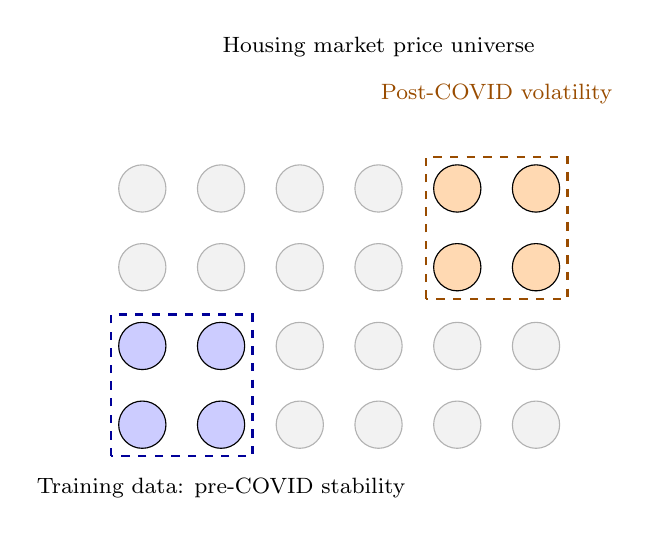
\begin{tikzpicture}[
      stable/.style={circle, draw=black, fill=blue!20, minimum size=0.6cm},
      covid/.style={circle, draw=black, fill=orange!30, minimum size=0.6cm},
      neutral/.style={circle, draw=black!30, fill=gray!10, minimum size=0.6cm},
      every node/.style={font=\scriptsize}
  ]
  
  % Grid layout (6x4)
  \foreach \x in {0,1,2,3,4,5} {
      \foreach \y in {0,1,2,3} {
          \node[neutral] (n\x\y) at (\x, \y) {};
      }
  }

  % Training data for stable market (left 2x2)
  \foreach \x in {0,1} {
      \foreach \y in {0,1} {
          \node[stable] at (\x, \y) {};
      }
  }

  % New dynamics during COVID (right 2x2)
  \foreach \x in {4,5} {
      \foreach \y in {2,3} {
          \node[covid] at (\x, \y) {};
      }
  }

  % Labels
  \node[align=left, font=\footnotesize] at (1, -0.8) {Training data: pre-COVID stability};
  \node[align=left, font=\footnotesize, text=orange!60!black] at (4.5, 4.2) {Post-COVID volatility};
  \node[align=left, font=\footnotesize] at (3, 4.8) {Housing market price universe};

  \draw[dashed, thick, blue!60!black] (-0.4, -0.4) rectangle (1.4, 1.4);
  \draw[dashed, thick, orange!60!black] (3.6, 1.6) rectangle (5.4, 3.4);

  \end{tikzpicture}
  \caption{Model Failure from Distributional Drift: Zillow’s prediction engine trained on pre-COVID stability (blue), but volatility emerged in unmodeled housing zones (orange).}
\end{figure}







